{
    \subsection{Տվյալների հավաքագրում}\label{subsec:dataCollection}
    Ծրագրային կոդի հատկությունների հարցումների համակարգի համար էական դեր ունի տվյալների հավաքագրման փուլը
    (Նկար \ref{fig:figure5}): Այս փուլում  կարևոր է տվյալներ հավաքագրող համակարգի
    օգտագործումը: Տվյալներ հավաքագրող համակարգի նպատակն է վերլուծել ծրագրային կոդը և հավաքագրել անհրաժեշտ
    տեղեկություններ՝ ներառյալ ծրագրի կառուցվածքի, ղեկավարման հոսքի և ներքին փոխկապակցվածությունների վերաբերյալ։

    \begin{figure}[h]
        \centering
        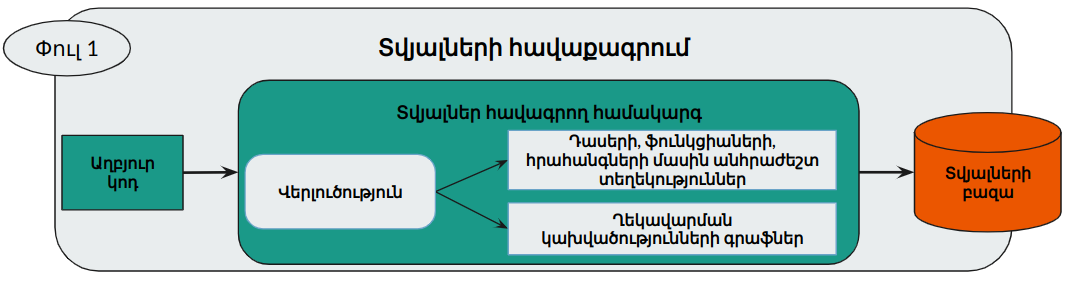
\includegraphics[width=1\textwidth]{pic5}
        \caption{Փուլ 1, տվյալների հավաքագրում}
        \label{fig:figure5}
    \end{figure}

    Տվյալներ հավաքագրող համակարգը մուտքում ստանում է աղբյուր կոդի ֆայլերը և իրականացնում վերլուծություններ՝
    ընդգրկելով հետևյալ տեղեկությունների հավաքագրումը.
    \begin{enumerate}
        \item Դասերի մասին տեղեկություններ՝ ներառյալ յուրաքանչյուր դասի անունը, դասի դաշտերը,
        աղբյուր կոդի տողերի համարները, ժառանգականության կապերը, ֆունկցիաները և այլն,
        \item Ֆունկցիաների մասին տեղեկություններ՝ ներառյալ յուրաքանչյուր ֆունկցիայի անունը, վերասահմանված ֆունկցիա լինելը,
        աղբյուր կոդի տողերի համարները, հայտարարող դասի անունը, կանչվող ֆունկցիաները, արգումենտները, լոկալ փոփոխականները,
        օգտագործվող և սահմանվող դաշտերը, տեսանելիությունը և այլն,
        \item Հրահանգների մասին տեղեկություններ՝ ներառյալ յուրաքանչյուր հրահանգների տիպը, աղբյուր կոդի տողերը,
        կանչվող ֆունկցիաները, օպերանդները, օգտագործվող և սահմանվող փոփոխականները և այլն:
    \end{enumerate}

    Այս տվյալները պահվում են կառուցված տվյալների բազայում՝ հետագա վերլուծությունների և հարցումների համար
    օգտագործելու նպատակով: Դրանք հիմք են հանդիսանում ծրագրային կոդի հատկությունների հարցումների համակարգի համար:

    {
    \subsubsection{Տվյալների բազայի նախագծում}\label{subsubsec:database}

    Հարցումները արդյունավետ կատարելու նպատակով տվյալների բազայի նախագծում՝ հաշվի առնելով ռելացիոն ու ոչ ռելացիոն
    բազաների հատկությունները։

    \begin{figure}[h]
        \centering
        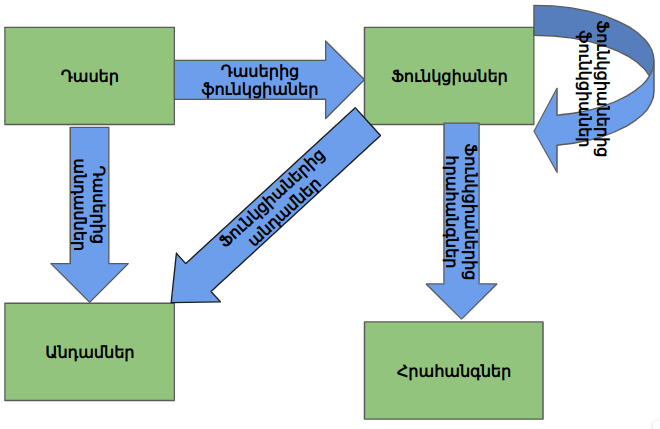
\includegraphics[width=0.8\textwidth]{pic7}
        \caption{Տվյալների բազայի կառուցվածքը}
        \label{fig:figure7}
    \end{figure}
}

%    {

}
}